\documentclass[11pt]{article}
\usepackage[a4paper,margin=2.2cm]{geometry}
\usepackage[T1]{fontenc}
\usepackage{lmodern}
\usepackage{graphicx}
\usepackage{caption}
\usepackage{amsmath}
\usepackage[hidelinks]{hyperref}

\renewcommand{\thefigure}{S\arabic{figure}}
\renewcommand{\thetable}{S\arabic{table}}

\title{\textbf{Supplementary Material}\\[4pt]
\large \emph{Catalogue of Catalogues}: A Web Platform for Earthquake
Catalogue Management, Merging, and Statistical Analysis}
\author{}
\date{}

\begin{document}
\maketitle
\vspace{-2.2\baselineskip}

\noindent
This supplement collects additional screen captures of the \emph{Catalogue of
Catalogues} (CofC) platform that support, but are not essential to, the argument
of the main paper.  All captures are from release \texttt{v0.1.0} running in a
browser against a local instance.

\medskip
\noindent
\textbf{Data.}  Every capture uses the reduced-scale synthetic catalogue pair
described in the main paper (a $5{,}200$-event ``GeoNet-like'' catalogue and a
$4{,}300$-event ``Agency~B'' catalogue, sharing a 50\,\% duplicate overlap),
generated with a fixed seed by the script in the source repository.  No real
event data are shown anywhere in this supplement.

\section*{Statistical analysis in the browser}

\begin{figure}[ht]
  \centering
  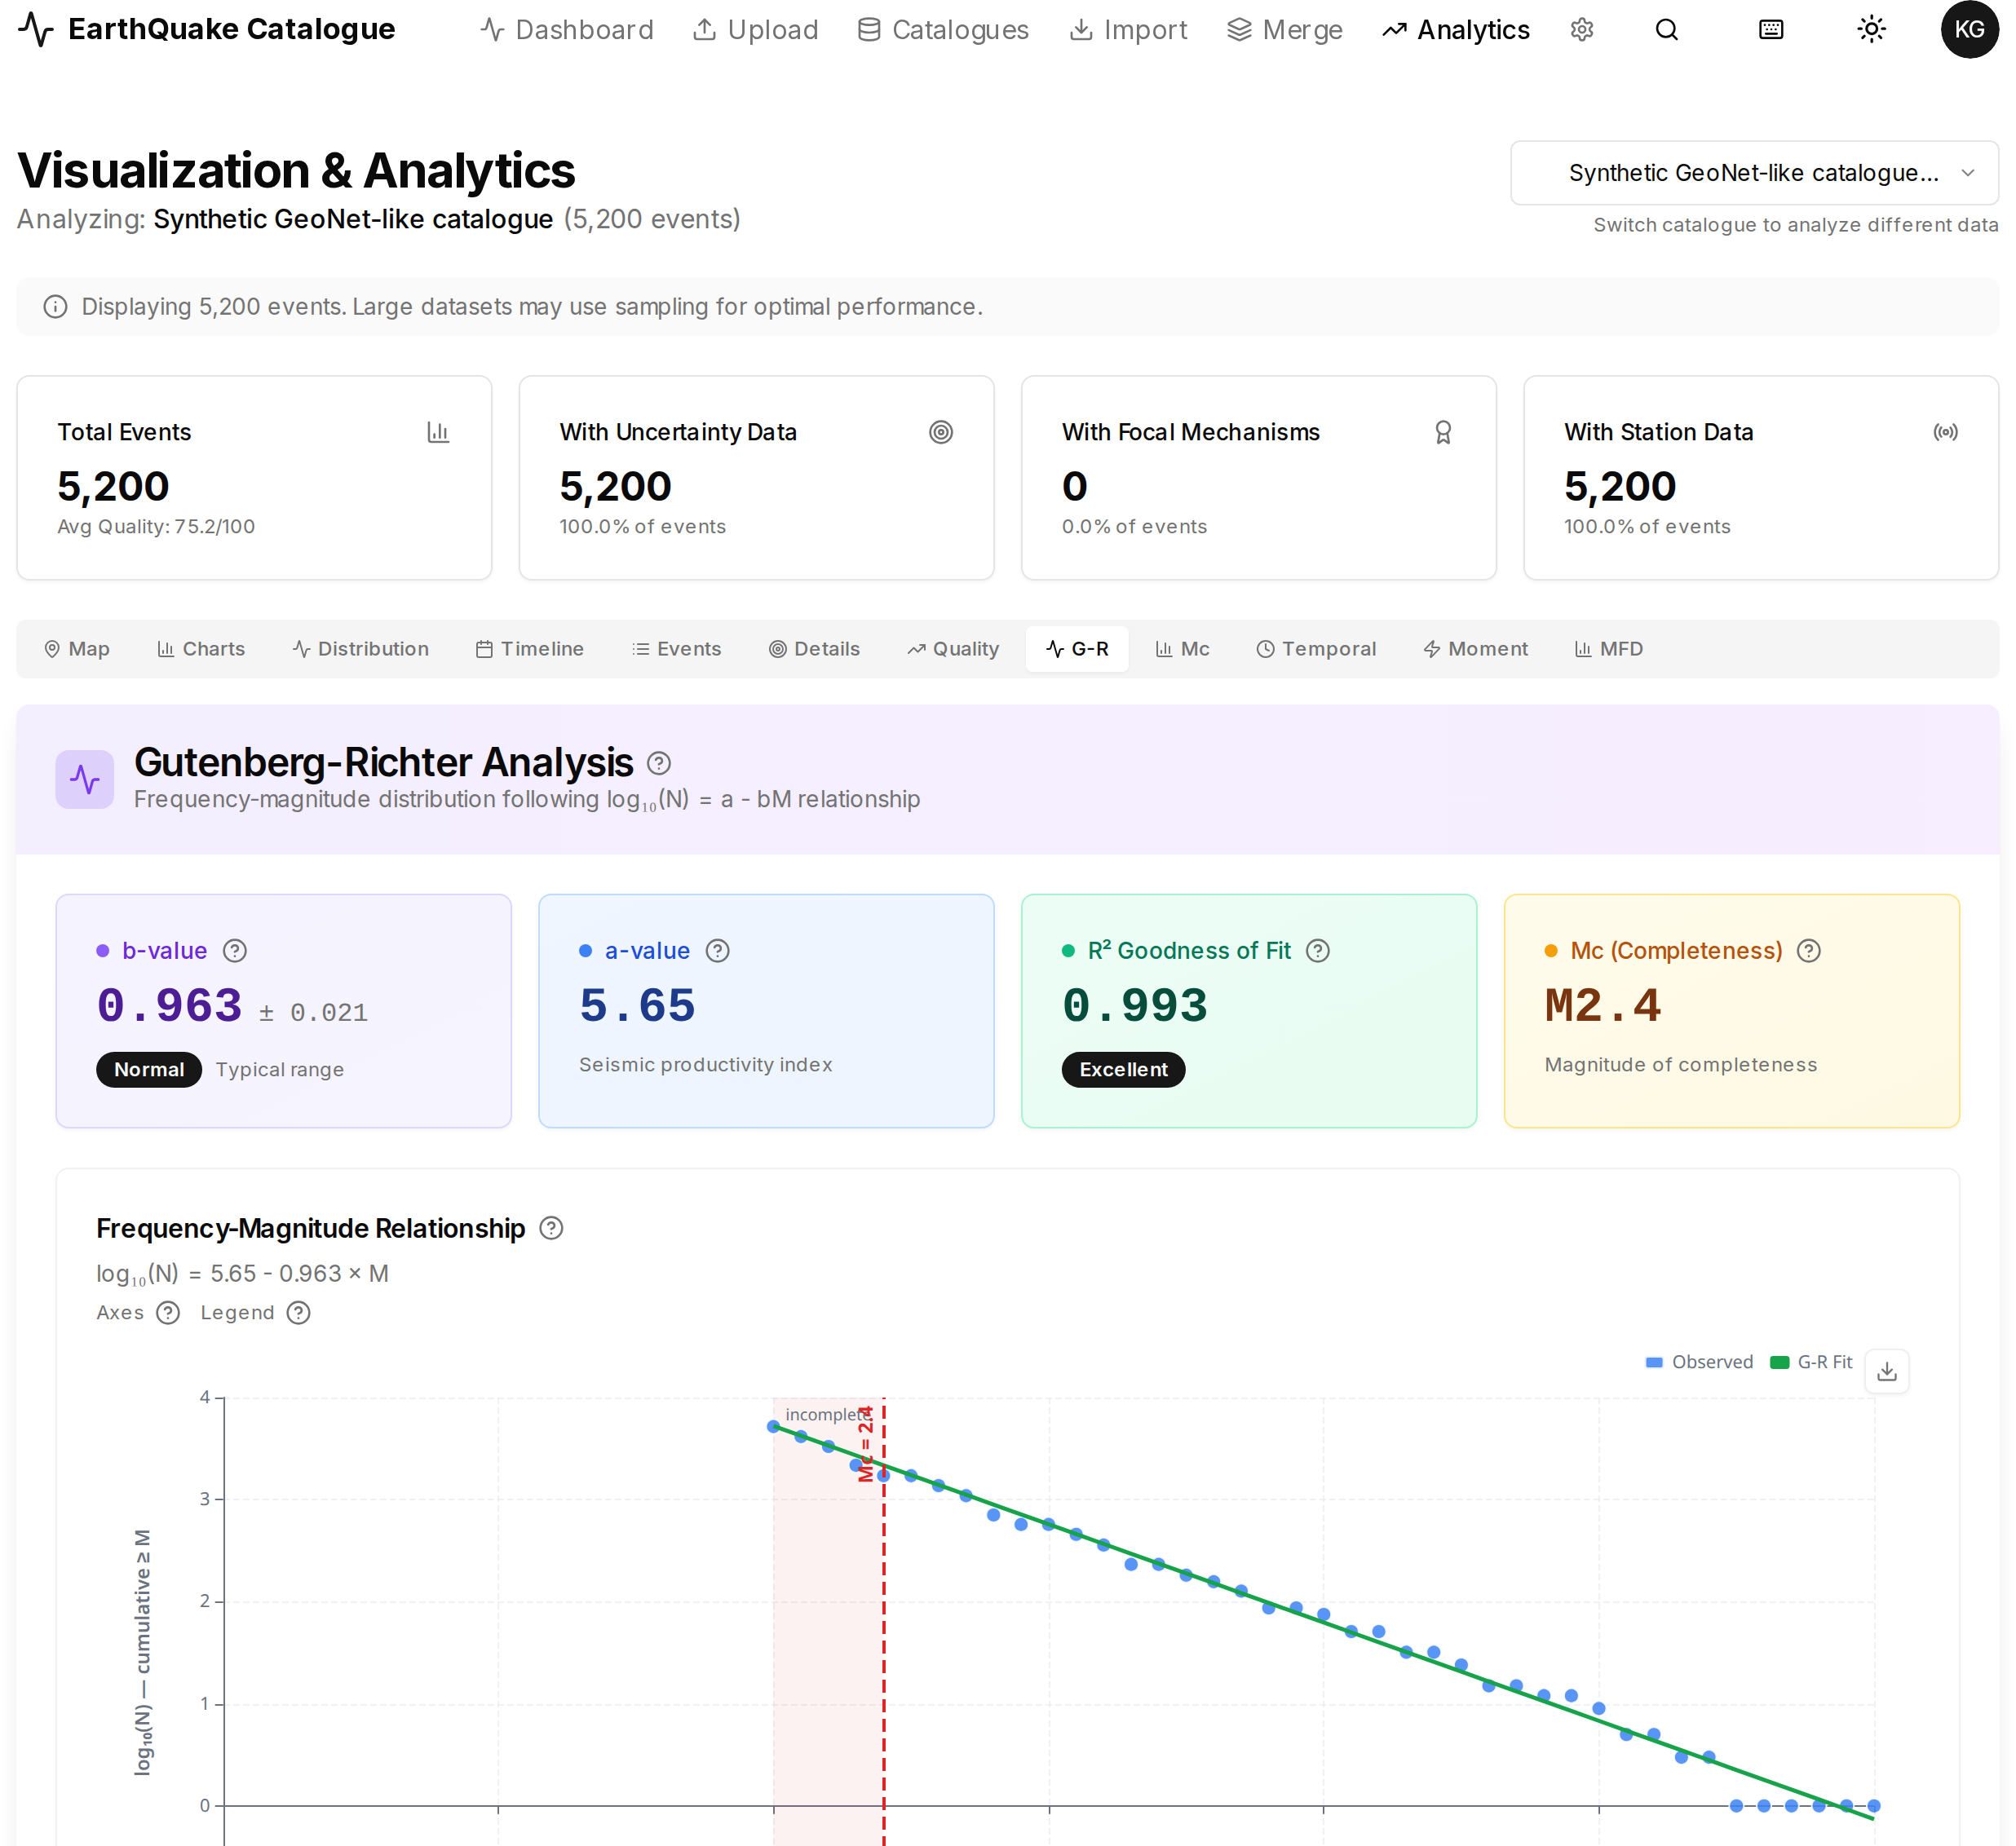
\includegraphics[width=\linewidth]{figures/app_analytics_gr_c.png}
  \caption{Gutenberg-Richter analysis of the synthetic GeoNet-like catalogue,
  computed client-side.  The platform reports $\hat{b}$ with its
  counting-statistics uncertainty, the $a$-value, the goodness of fit, and the
  Maximum Curvature estimate of $M_c$; the frequency-magnitude plot marks the
  incomplete range below $M_c$ and overlays the fitted relation.  The recovered
  $\hat{b} = 0.963 \pm 0.021$ is consistent with the $b = 1.0$ used to generate
  the synthetic catalogue, and is a check on the estimator rather than a
  measurement of New Zealand seismicity.}
  \label{fig:s_gr}
\end{figure}

\begin{figure}[ht]
  \centering
  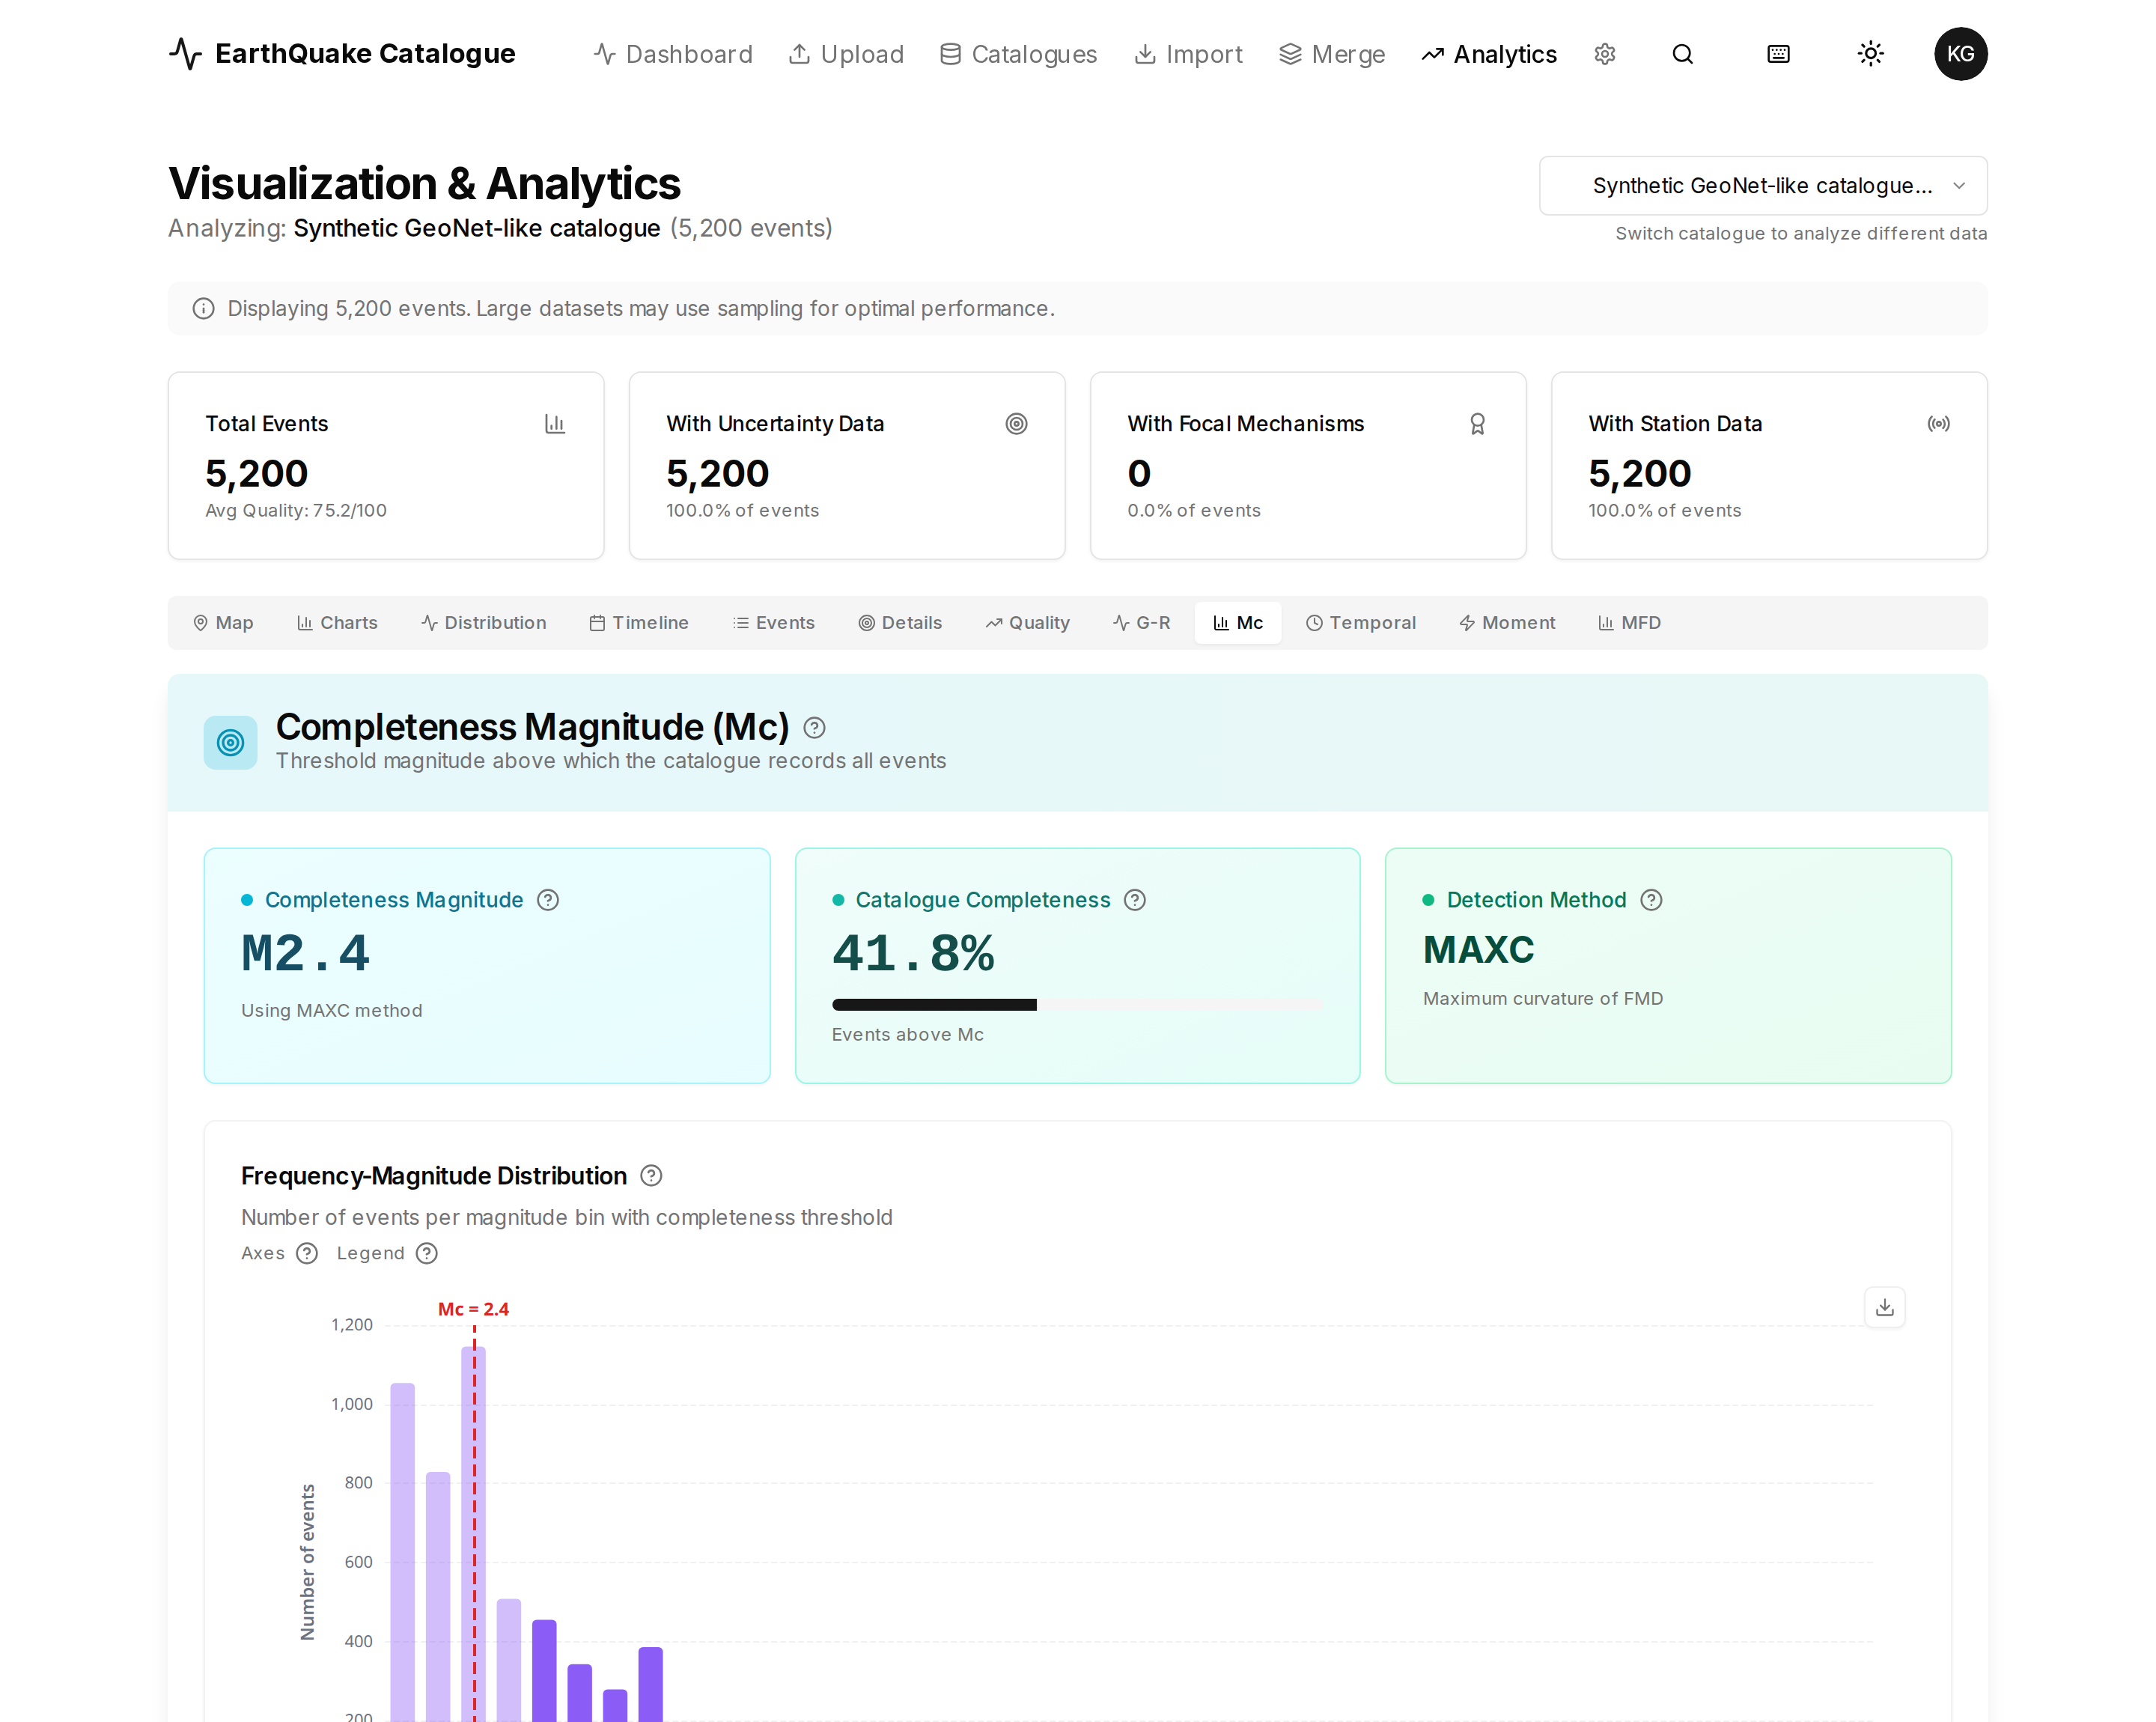
\includegraphics[width=\linewidth]{figures/app_analytics_mc.png}
  \caption{Magnitude-of-completeness panel for the same catalogue.  $M_c$ is
  estimated by Maximum Curvature with the $+0.2$ correction discussed in the
  main paper, and is exposed as an explicit, user-adjustable cut-off rather than
  applied silently, so that the completeness assumption behind any subsequent
  $b$-value is visible at the point of use.}
  \label{fig:s_mc}
\end{figure}

\section*{Event-level quality index}

\begin{figure}[ht]
  \centering
  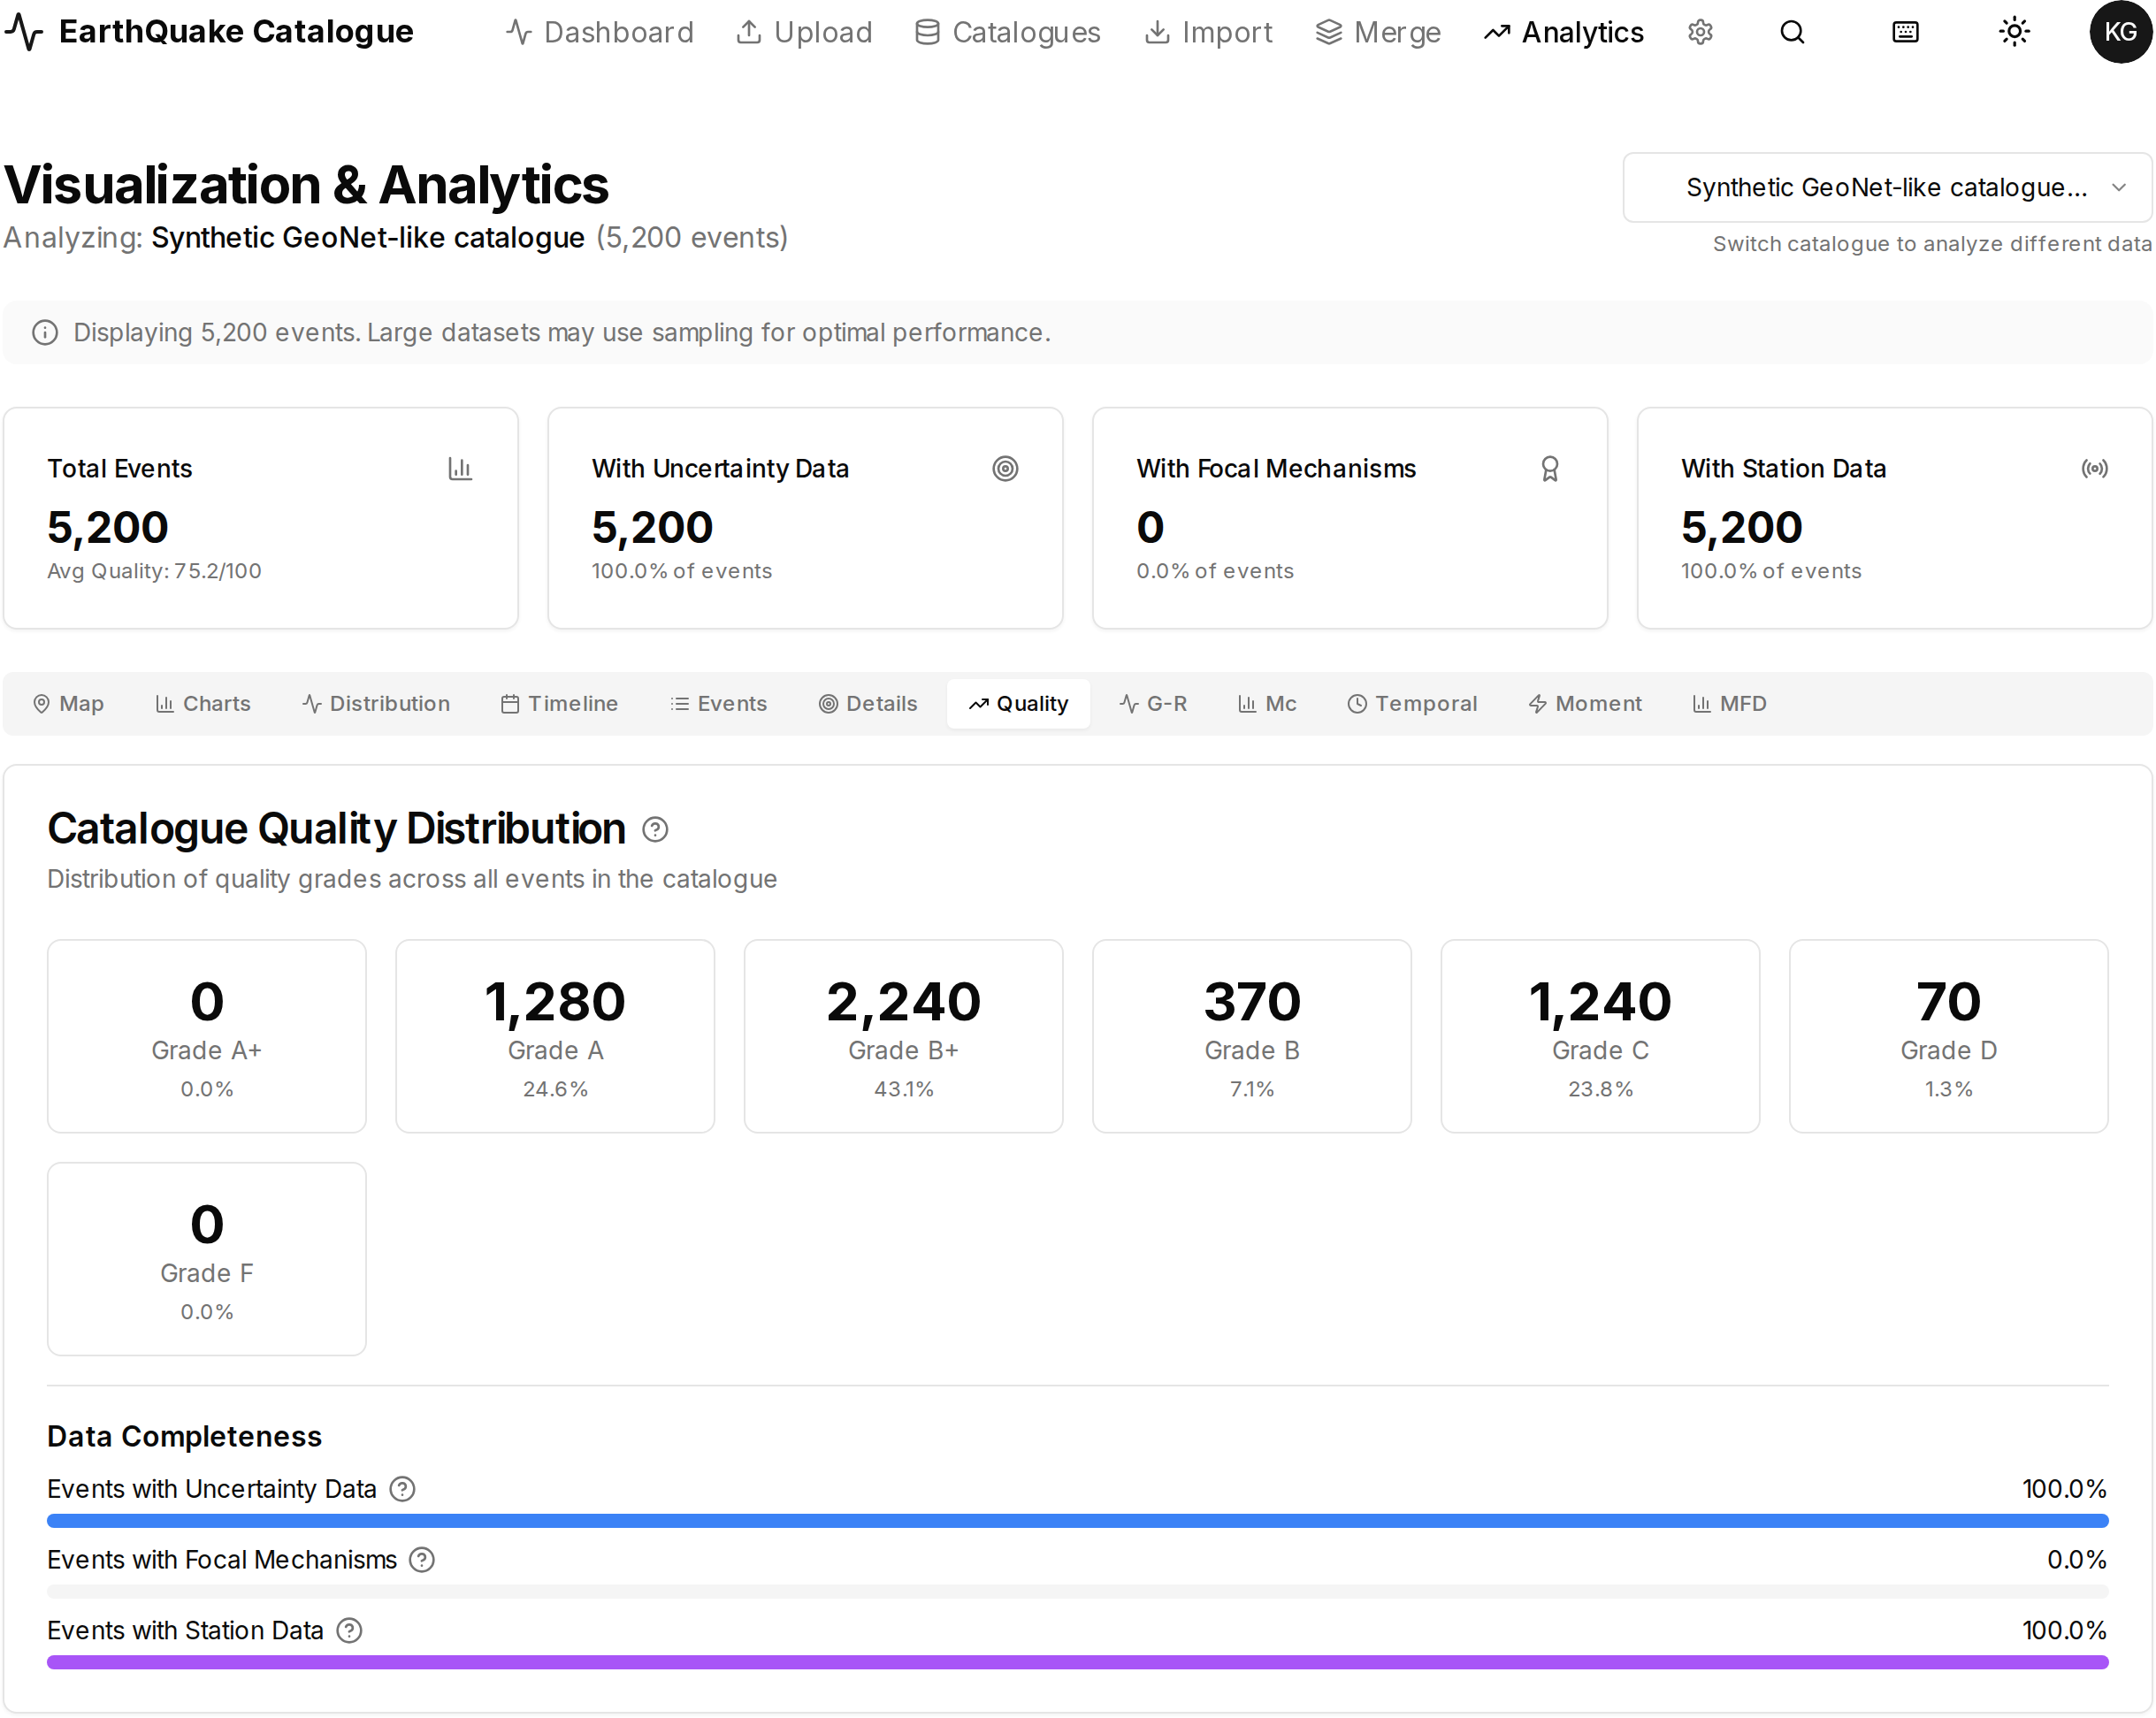
\includegraphics[width=\linewidth]{figures/app_analytics_quality_c.png}
  \caption{Catalogue-level summary of the per-event quality index
  (equation~1 of the main paper) for the synthetic GeoNet-like catalogue.  Every
  event is scored on import and mapped to an A\textsuperscript{+}--F grade; the
  panel reports the grade distribution and the mean score, together with the
  field-completeness fractions that feed the individual sub-scores.  The absence
  of focal mechanisms in this synthetic catalogue is reflected in the
  completeness bars, and depresses the achievable score, which is why no event
  reaches grade~A\textsuperscript{+}.}
  \label{fig:s_quality}
\end{figure}

\end{document}
